% !TEX root = ../main.tex
% Chapter --- Verification at Independent Stations
\chapter{Verification at Independent Stations}\label{ch:stations}
In this chapter we compare selected results of  \cref{ch:single-model} to real measurements at weather stations. The target fields the model trained on are MeteoSwiss analyses, which are
themselves interpolated from station observations \cite{meteoswiss_ogd_grid} so the measurements are not completely independent. Three station sets
are used (\tref{tab:stations-sets}). All are MeteoSwiss open data, cover 2020--2024, and entered in this form no
training or model-selection step of this work: the homogenised daily temperature maxima of $28$ stations of the
Swiss National Basic Climatological Network (NBCN)~\cite{begert2005homogeneous,meteoswiss_ogd_nbcn},
the operational daily temperature maxima of $147$ SwissMetNet (SMN) stations, and the daily totals of $139$ SMN
rain gauges~\cite{meteoswiss_ogd_smn}.

\begin{table}[H]
\centering
\caption[Reference Meteorological Observations at Stations]{Three sets of observation station used for verification. A station enters its
set if it reports on at least $95\,\%$ of the days in 2020--2024; the day labelling of every series
was verified against its gridded counterpart before scoring (\sref{sec:app-stations}).}
\label{tab:stations-sets}
\footnotesize
\setlength{\tabcolsep}{4pt}
\begin{tabular}{|p{2.2cm}|p{1.5cm}|p{4.6cm}|p{2.2cm}|p{3.2cm}|}
\hline
\textbf{Set} & \textbf{Stations} & \textbf{Observable} & \textbf{Series} & \textbf{Verifies} \\
\hline
NBCN & $28$ & daily maximum $2\,\mathrm{m}$ temperature & homogenised & \texttt{atm+wind-clip60} \\
\hline
SMN temperature & $147$ & daily maximum $2\,\mathrm{m}$ temperature & operational & \texttt{atm+wind-clip60} \\
\hline
SMN rain gauges & $139$ & daily precipitation, $06$--$06\,\mathrm{UTC}$ & operational & \texttt{precip-FT-CRPS}, \texttt{precip-SFC-TP} \\
\hline
\end{tabular}
\end{table}

No regridding is involved in this comparison. The RBF final layer of \sref{subsec:meth-backbone}
decodes the predictive distribution at the station coordinates directly, so no gridded prediction is
resampled and no observation is interpolated. The gauge series is the $06$--$06\,\mathrm{UTC}$ daily
total, the accumulation window RhiresD itself uses \cite{meteoswiss_rhiresd_doc}. The reference at a
station is the same bilinear ERA5-Land interpolation as in \cref{ch:single-model}. 

\section{Temperature}\label{sec:stations-tmax}

\begin{figure}[H]
\centering
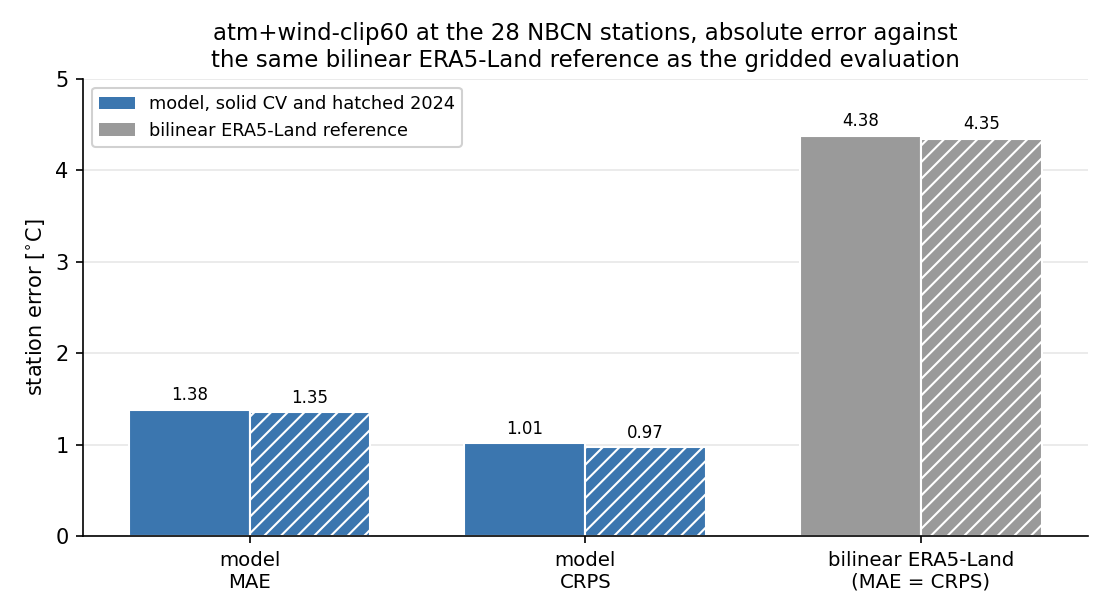
\includegraphics[width=\textwidth]{images/stations/tmax_selected_station_abs.png}
\caption[Verification at the 28 NBCN stations]{The selected temperature model at the $28$ NBCN
stations, solid bars for the CV holdout and hatched for 2024: the model's MAE and CRPS in physical
units, beside the bilinear ERA5-Land reference of \cref{ch:single-model}. The reference is
deterministic, so its CRPS equals its MAE and one bar serves both.}
\label{fig:stations-tmax-abs}
\end{figure}

The station comparison returns the verdict of \sref{subsec:single-tmax-geography}, and the
generalisation pattern of \fref{fig:single-tmax-slope} repeats at the measurement points:
\texttt{atm+wind-clip60} improves from $1.38$ to $1.35\,^{\circ}\mathrm{C}$ MAE between the CV
holdout and the unseen year (\fref{fig:stations-tmax-abs}). Station errors sit roughly
$0.3\,^{\circ}\mathrm{C}$ above their gridded counterparts throughout. In physical units the model reaches a station CRPS of $1.02$ and
$0.97\,^{\circ}\mathrm{C}$ against the $4.38$ and $4.35\,^{\circ}\mathrm{C}$ of the raw bilinear
reference, less than a quarter of the interpolation error in either regime. The pooled skill of
$0.77$ and $0.78$ is consistent with the gridded skill of $0.70$ and $0.71$ of \sref{subsec:single-tmax-unseen}\footnote{ \sref{subsec:single-tmax-unseen} already showed the
model scoring highest exactly where the reference fails, and at a station the reference is
handicapped further: it interpolates ERA5-Land to the station coordinates but not to the station
elevation, so at an alpine site much of its error is the unresolved elevation itself. The station
skill is therefore best read as confirmation of the gridded evaluation at real measurement points,
not as an absolute measure of the margin over interpolation.}.



\begin{figure}[H]
\centering
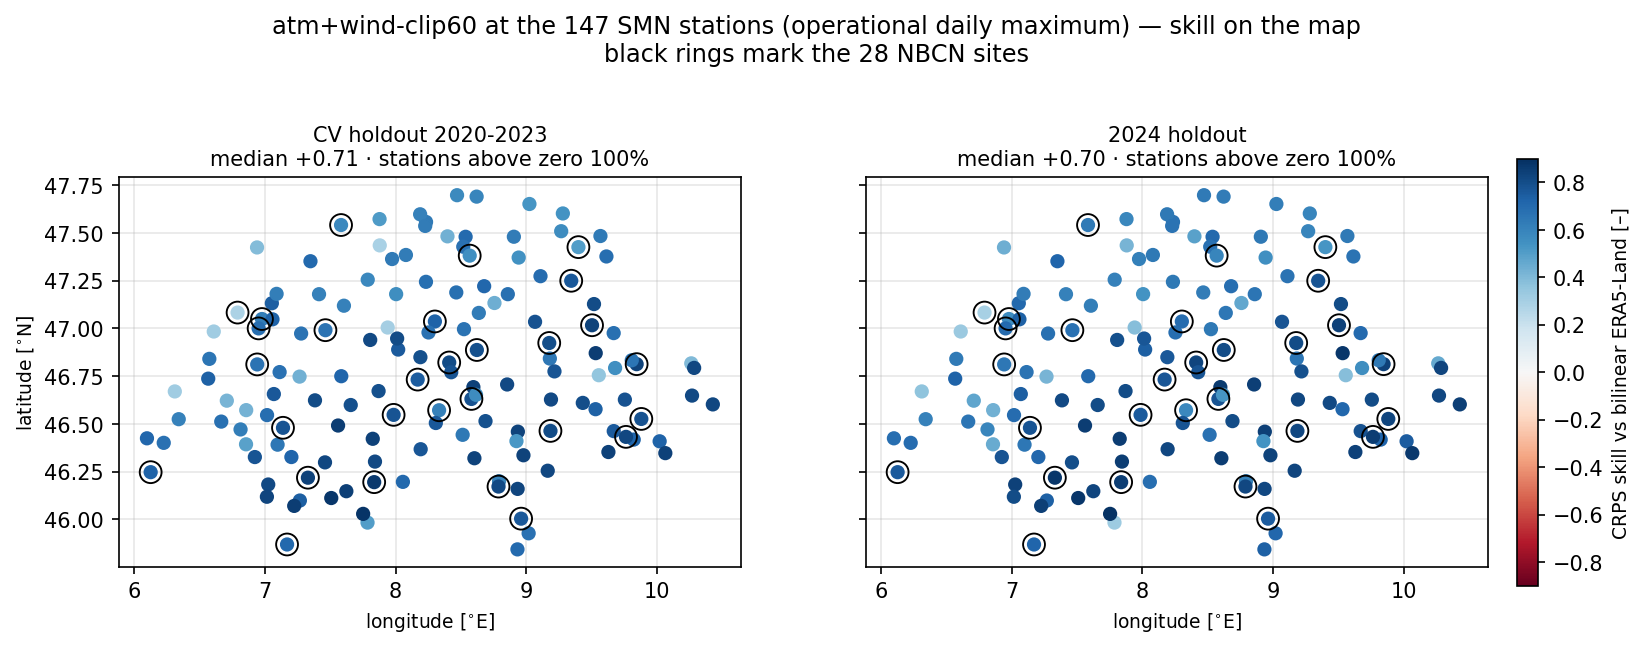
\includegraphics[width=\textwidth]{images/stations/tmax_station_skill_map_raw.png}
\caption[Skill at the 147 SMN stations]{Per-station CRPS skill of \texttt{atm+wind-clip60} against
the bilinear ERA5-Land reference at the $147$ SMN stations, under both regimes; black rings mark
the $28$ NBCN sites. The median station reads $+0.71$ and $+0.70$, and every station is above zero
in both regimes.}
\label{fig:stations-tmax-map}
\end{figure}

The claim survives breadth as well as quality. Widening the analysis from the $28$ homogenised NBCN
series to the $147$ SMN stations reporting the operational daily maximum confirms the model's superiority over interpolation: it reaches a station
MAE $1.41$ and $1.39\,^{\circ}\mathrm{C}$ across the two regimes, a median skill of $+0.71$ and
$+0.70$, and every station above zero (\fref{fig:stations-tmax-map}). At the
$28$ sites the two cohorts share, the operational and homogenised series give per-station errors
that agree to a median of $0.00\,^{\circ}\mathrm{C}$ over this span, so the distinction between the
two series carries no weight here. The model therefore beats interpolation at every real
measurement point it was tested on. 

\section{Precipitation}\label{sec:stations-precip}

For precipitation this comparison
sharpens the conclusions of \sref{sec:single-precipitation}. The
occurrence prediction of the bilinear ERA5-Land fails: it identifies half of all days as
wet ($0.50$ against an observed frequency of $0.33$ on the CV holdout), while both selected runs
stay within $0.05$ of the observed frequency in both regimes. This is the station-level counterpart
of the R01 result of \fref{fig:precip-indices}.

\begin{figure}[H]
\centering
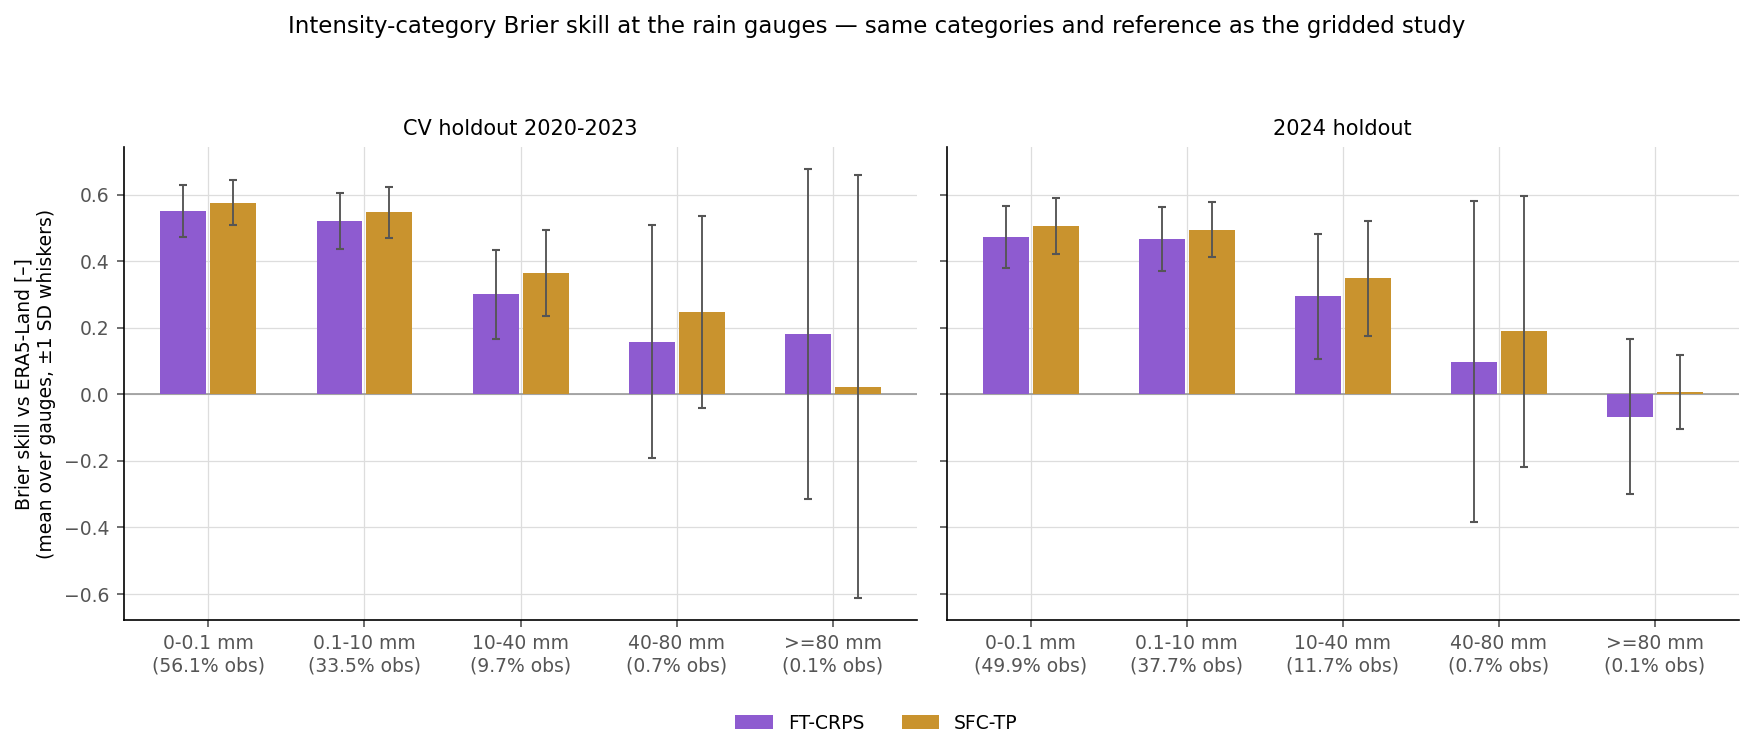
\includegraphics[width=\textwidth]{images/stations/precip_category_bss.png}
\caption[Intensity-category Brier skill at the rain gauges]{Brier skill against the bilinear
ERA5-Land reference at the $139$ gauges, by intensity category, the same categories and reference
construction as \fref{fig:single-precip-categories}. For each category, the bar shows the mean of
the per-gauge Brier skills and the whisker their $\pm 1$ standard deviation across gauges, a spread
rather than a standard error; the observed frequency of the category is noted beneath it.}
\label{fig:stations-precip-bss}
\end{figure}

Scored by intensity category, the gauges reproduce the gridded structure of
\sref{subsec:single-precip-categories} (\fref{fig:stations-precip-bss}). Skill falls
with intensity for both runs, and \texttt{precip-SFC-TP} leads in every category that carries an
appreciable share of days, exactly as in the gridded ordering. The mean skill stays positive
through the $40$--$80\,\mathrm{mm}$ category ($+0.25$ and $+0.19$ for \texttt{precip-SFC-TP},
$+0.16$ and $+0.10$ for \texttt{precip-FT-CRPS}, across the two regimes) and is indistinguishable
from zero at $\geq 80\,\mathrm{mm}$, where the whiskers span both signs. The heaviest events remain
the limit of what these models deliver, at the gauges as on the grid.

The surface-based run is ahead of the free-troposphere run at every category below $80\,\mathrm{mm}$, in both regimes. The advantage is small but consistent. However as the gridded evaluation is not independent of the station verification, this does not contradict the conclusion of \sref{sec:single-precipitation}. The station verification is a confirmation of the gridded evaluation, not an independent assessment of the two runs against each other. 

\begin{figure}[H]
\centering
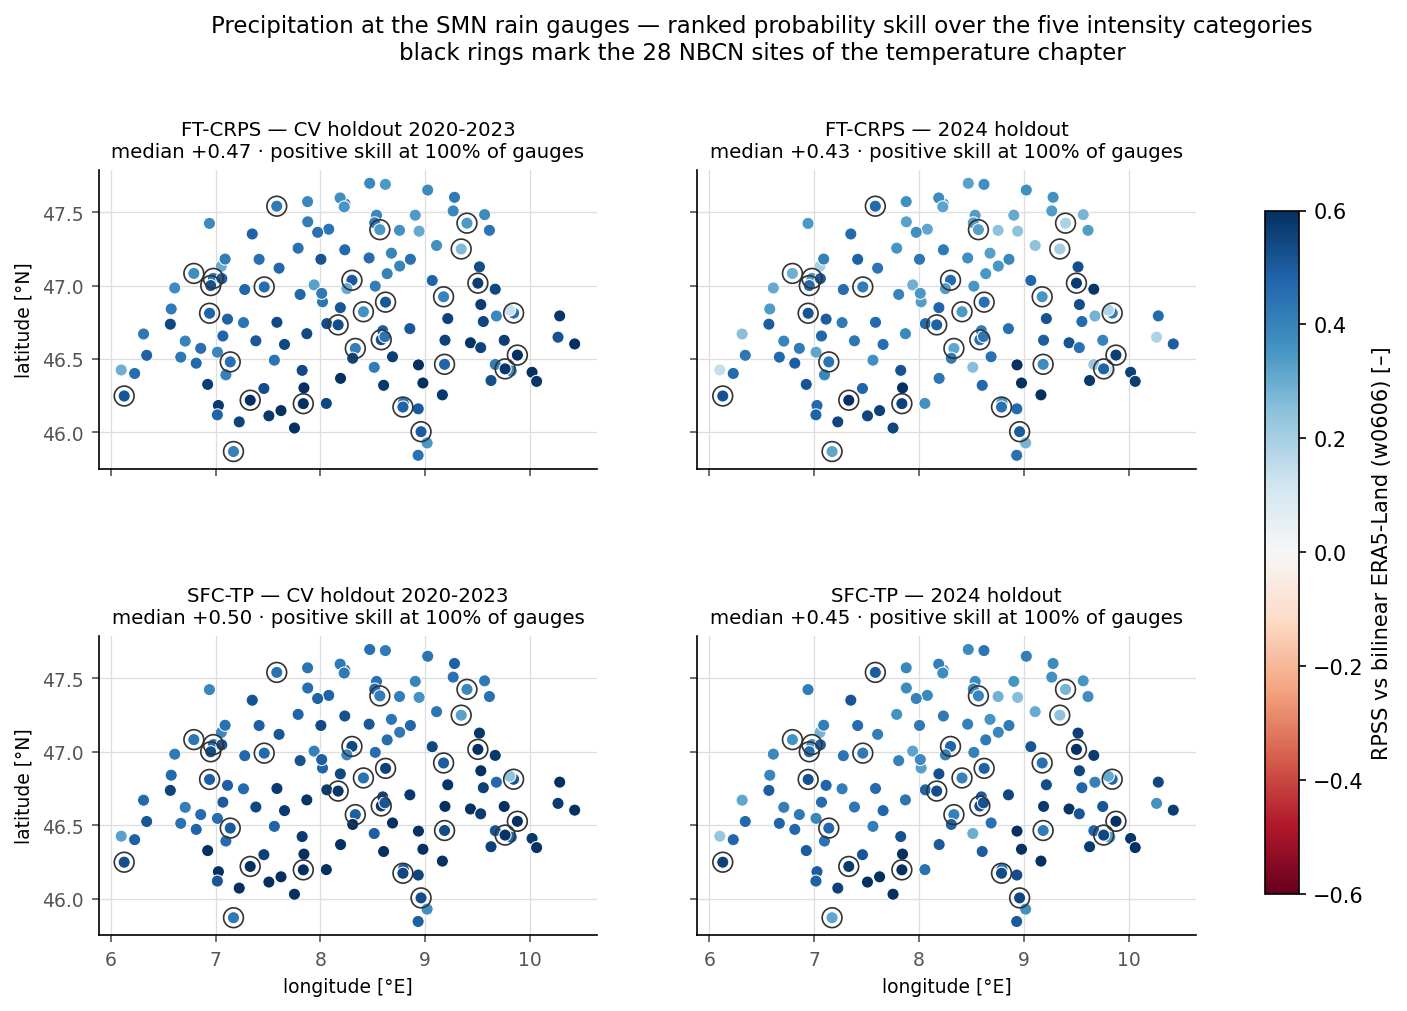
\includegraphics[width=\textwidth]{images/stations/precip_gauge_skill_map.png}
\caption[Ranked probability skill at the 139 rain gauges]{Per-gauge ranked probability skill over
the five intensity categories, against the bilinear ERA5-Land reference, for both selected runs and
both regimes; black rings mark the $28$ NBCN sites.}
\label{fig:stations-precip-map}
\end{figure}


Pooled over the categories, both runs beat plain interpolation at every one of the $139$ gauges, in
both regimes: the median ranked probability skill is $+0.50$ and $+0.45$ for
\texttt{precip-SFC-TP} and $+0.47$ and $+0.43$ for \texttt{precip-FT-CRPS}
(\fref{fig:stations-precip-map}). 

\begin{figure}[H]
\centering
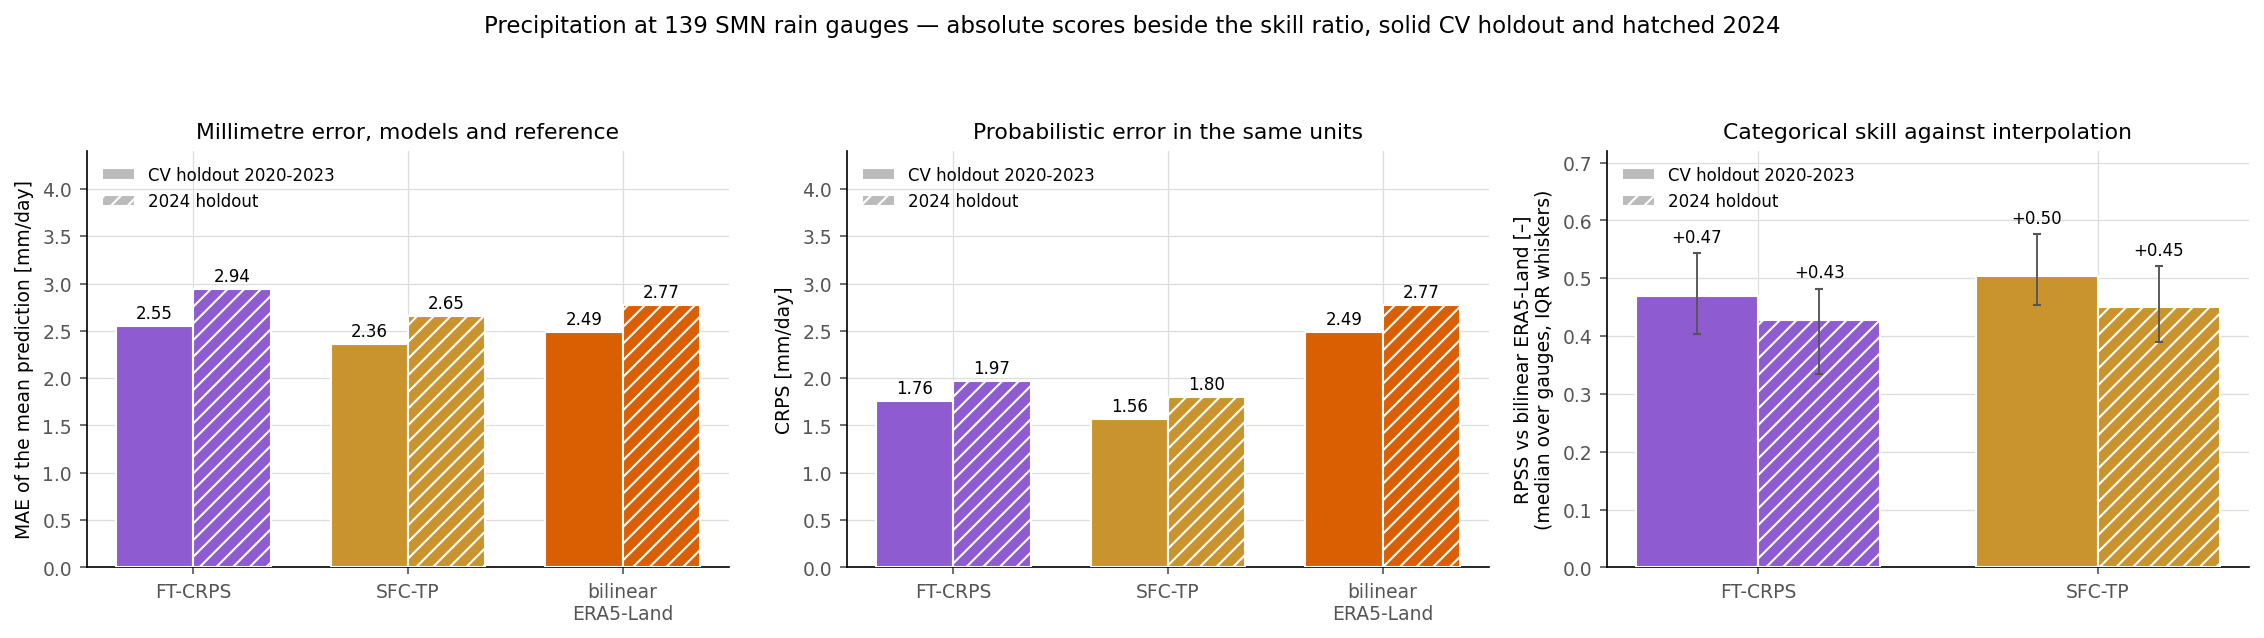
\includegraphics[width=\textwidth]{images/stations/precip_absolute_values.png}
\caption[Absolute scores at the rain gauges]{The two selected precipitation runs at the $139$
gauges, solid bars for the CV holdout and hatched for 2024. Left: MAE of the mean of the predicted
distribution. Middle: CRPS of the full distribution, in the same units; the reference carries no
distribution, so its CRPS is its MAE and the same bar serves both panels. Right: the median
per-gauge ranked probability skill, with interquartile whiskers.}
\label{fig:stations-precip-abs}
\end{figure}

\fref{fig:stations-precip-abs} restates the gauge verification in absolute units, since a ranked
probability skill of $+0.50$ says nothing about the size of the errors underneath it. The millimetre
picture remains a near-tie, with one shift of sign against \fref{fig:single-precip-slope-skill}:
scored as a point forecast through the mean of its predicted distribution, \texttt{precip-SFC-TP} performs ahead of the reference ($2.36$ and $2.65\,\mathrm{mm\,day^{-1}}$ against $2.49$ and
$2.77$ across the two regimes; the reference is scored at the gauges here, so these are not the
$2.29\,\mathrm{mm}$ it reaches on the gridded target), where on the grid it was marginally behind, while
\texttt{precip-FT-CRPS} stays behind at $2.55$ and $2.94$. A plausible reason is the target itself:
the gridded truth is an interpolated, smoothed field, which flatters a smooth reference in a
pointwise score, whereas a real gauge series is rougher and penalises it. Scored as distributions, both runs are clearly ahead, at a CRPS of
$1.56$ and $1.80\,\mathrm{mm\,day^{-1}}$ for \texttt{precip-SFC-TP} and $1.76$ and $1.97$ for
\texttt{precip-FT-CRPS}, between $29$ and $37\,\%$ below the reference in every case. The whole
panel shifts upward from the CV holdout to 2024, the reference included, so the deterioration on the
unseen year belongs at least partly to the year rather than to the models.
